\documentclass{llncs}
%
\usepackage{makeidx}  % allows for indexgeneration
\usepackage[british]{babel}
\usepackage{graphicx}
\usepackage{tabularx}
\usepackage{subcaption}
\usepackage{listings}
\usepackage{url}
\usepackage[pdftex,colorlinks=true]{hyperref}
%\fussy

% global options for listings package
\lstset{breaklines=true,breakatwhitespace=true,showstringspaces=false,basicstyle=\ttfamily\footnotesize}

\title{Changing Faces: Identifying Complex Behavioural Profiles}
\author{Giles Oatley and Tom Crick}
\institute{Department of Computing \& Information Systems\\
Cardiff Metropolitan University\\
Cardiff CF5 2YB, UK\\
\email{\{goatley,tcrick\}@cardiffmet.ac.uk}
}

\raggedbottom
\begin{document}
%
\frontmatter          % for the preliminaries
%
\pagestyle{headings}  % switches on printing of running heads
%\addtocmark{} % additional mark in the TOC

% fix listings numbering from "Chapter.Num." to just "Num."
% e.g. the first one was numbered 1.1. rather than 1.
\renewcommand{\thelstlisting}{\arabic{lstlisting}}

\maketitle

\begin{abstract}
There has been significant interest in the identification and
profiling of insider threats, attracting high-profile policy focus and
strategic research funding from governments and funding bodies.
Recent examples attracting worldwide attention include the cases of
Chelsea Manning, Edward Snowden and the US authorities. The challenges
with profiling an individual across a range of activities is that
their data footprint will legitimately vary significantly based on
time and/or location. The insider threat problem is thus a specific
instance of the more general problem of profiling complex
behaviours. In this paper, we discuss our preliminary research models
relating to profiling complex behaviours and present a set of
experiments related to changing roles as viewed through large-scale
social network datasets, such as Twitter. We employ psycholinguistic
metrics in this work, considering changing roles from the standpoint
of a trait-based personality theory.  We also present further
representations, including an alternative psychological theory (not
trait-based), and established techniques for crime modelling,
spatio-temporal and graph/network, to investigate within a wider
reasoning framework.
\end{abstract}

\section{Introduction}\label{intro}

The motivation for this preliminary research is a long-standing
interest in determining personality and behaviour from digital data
and especially profiling insider threats, a situation where granted
access is used illegitimately, often in situations where it is known
that actions are scrutinised closely (such as by machine learning
algorithms). How best then to develop a profile of an individual (we
do not consider group behavior in this paper) so that criminal
behavior, which is assumed to be different in some way to normal
operating behaviour, can be detected. The data footprint will vary
significantly based on either time, location or role, as the
individual legitimately passes through their range of activities; for
instance, an operator accessing a computer terminal at one location in
the morning and another in the afternoon. Likewise, the data footprint
will change according to shifting emotional states; for instance, the
same operator working at a single terminal differently on different
days, one day performing the `harder' tasks first, and another day,
the `easier' tasks first. Thus, we have the general problem of
profiling complex behaviours.

From collaborations with several UK police forces and crime prevention
partnerships, we have seen a wide range of data and problems, with the
need to develop models with predictive or classification power,
embedded in decision support systems, namely: gun gangs, terrorism
networks, retail crime gangs, volume crime, fraud and sex offences.
Each problem collected different data, and therefore different
techniques were more appropriate to model the criminal behaviour.

Recent research suggests that it may be possible to identify
personality traits through textual analysis, that is, analysis of the
style and nature of an individuals written expression. A person's
identity or personality is reflected in everything they do, including
website design~\cite{vazire+gosling:2004} and textual communication on
the Internet more generally. The growth of social networking websites
has put an enormous amount of such written expressions into the public
domain for the first time, and investigators have presented frameworks
for forensic treatment of this data~\cite{haggerty-et-al:2012}.
Included in our study, we present an unreported set of experiments
related to changing roles as viewed through Twitter social media data.

Attempts to characterise personality typologies, include McAdams'
intuitively appealing model~\cite{adams:1996} with the three levels of
({\emph{i}}) traits, ({\emph{ii}}) mental concerns and strategies
(intermediate knowing), and ({\emph{iii}}) life story (intimate
level). Gosling~\cite{gosling:2009} describes the trait level as
painting a portrait in broad brushstrokes but which leaves out much of
the finer detail. An example of a trait model is the Big Five or Five
Factors (as used in our study), namely: extraversion, emotional
stability, agreeableness to other people, conscientiousness and
openness to experience~\cite{costa+mccrae:1992,norman:1963}. There are
many ways to be extraverted for instance, and what are these traits
able to tell us about a person's values, beliefs, goals and roles;
these are the next level of knowing someone. Having worked through the
traits and personal concerns of McAdams’ first two levels, you strike
the bedrock of personality -- identity. McAdams describes this third
level as ``{\emph{an inner story of the self that integrates the
reconstructed past, perceived present, and anticipated future to
provide a life with unity, purpose, and meaning.}}''

For many operational purposes McAdams' lower level of traits can often
be sufficient, and certainly, because of its extensive use, it
provides a way of comparing research; over the last 50 years the Five
Factor model has become a standard in
psychology~\cite{mairesse-et-al:2007}, developing a large body of
research for comparison.

\section{Geospatial, Network and Modus Operandi Data}\label{geospatial}

Working with burglary data from West Midlands
Police~\cite{oatley+ewart:2003,oatley-et-al:2006a,oatley-et-al:2006b}
in the UK, several new methods were developed, including the composite
of geographical range and network connections as shown in
Figure~\ref{fig:geonets}. Each `square' is an offender, associated by
co-defendant (arrested together) links to other offenders. The map for
each offender shows their geographic range of offending. Each offender
also had a list of property stolen against each of their crimes, and
modus operandi (see Table~\ref{tab:burgdwellingsmo}), upon which it
was possible to develop predictive models.

\begin{figure}[!ht]
\centering
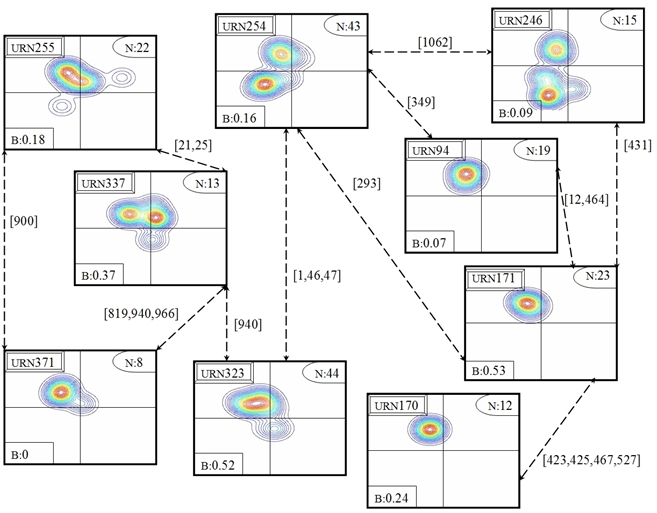
\includegraphics[width=0.9\columnwidth]{images/GeographicalNetworks.jpg}
\caption{{\textbf{Geographical networks.}} Each box is an offender, displaying their codefendent links, and geographical range of offending.}
\label{fig:geonets} 
\end{figure}

%%% Insert Table 1 here
\begin{table}[htb]
\centering
%\resizebox{0.9\textwidth}{!}{%
\begin{tabularx}{\textwidth}{|X|X|}
\hline
 LOCATION OF ENTRY &  1. Wall 2. Adjoining Property 3. Below, 4. Front
 5. Rear 6. Side7. Roof 8. Window 9. Door 10. Above \\
\hline 
 ENTRY METHODS AND BEHAVIOUR & 1. Smash 2. Cut 3. Cutting equipment
 4. Duplicate Key 5. Drill 6.Force 7. Remove Glass 8. Ram 9. Insecure
 door/window 10. Climbed \\
\hline
 TYPE OF DWELLING & 1. Old 2. Terrace 3. Maisonette 4. Bungalow
 5. Semi-detached 6. Town House 7. Flat \\
\hline
 SEARCH BEHAVIOUR & 1. Untidy Search 2. Downstairs Only 3. Many Rooms
 4. Upstairs Only 5. Tidy Search 6. Search All Rooms \\
\hline
 LOCATION OF EXIT & 1. Wall 2. Adjoining Property 3. Below 4. Front
5. Rear 6. Side 7. Roof 8. Window 9. Door 10. Exit Same as Entry \\
\hline
 ALARM/PHONE & 1. Cut Phone 2. Tamper with Alarm 3. Alarm Activated \\
\hline
 BOGUS OFFICIAL CRIME & 1. Social Services 2. Bogus Official (type
 unknown) 3. Council 4. DSS 5. Home Help 6. Gardener 7. Other 8. Water
 \\
\hline
\end{tabularx}%}
\caption{Burglary from dwelling house -- modus operandi features.}
\label{tab:burgdwellingsmo}
\end{table}

The modus operandi data was routinely gathered by scenes of crime
officers (SOCOs), and contained a range of `styles' of burgling, using
force or craft and so on~\cite{ewart+oatley:2003}.  A crucial
recommendation to West Midlands Police was that the SOCOs would record
richer data that could more adequately distinguish between obviously
different crime locations and perpetrators, in order to infer
behaviours and traits.

% Gang-related crime with Greater Manchester Police received a wide
% range of technologies~\cite{oatley+crick:unpub}. 

Ewart \& Oatley~\cite{ewart+oatley:2003} compared models that used
just spatio-temporal data (including correlated walk analysis) against
modus operandi, and a combination of both. The combined models
performed best. Figure~\ref{fig:offvictrips} shows a geographical plot
with triples of [\emph{offender home address, location, victim home
address}] for a range of crime types, including woundings, murder,
manslaughter, kidnapping and firearms offences. Representing the data
in this way, we are able (as in the previous geographical network) to
see offending characteristics such as criminal range, and
relationships between crime types.

\begin{figure}[!ht]
\centering
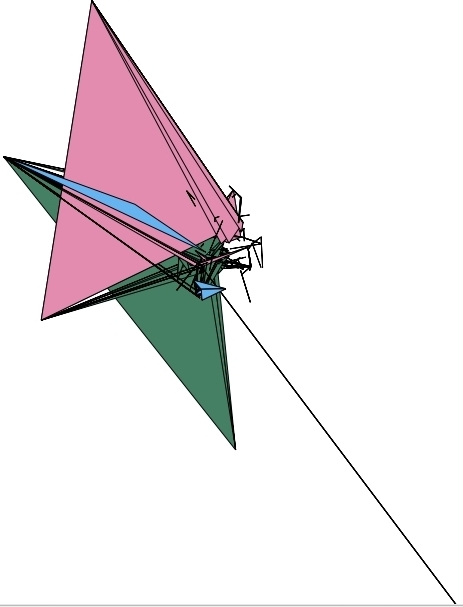
\includegraphics[width=0.6\columnwidth]{images/OffenderVictimOffenceTriples.jpg}
\caption{{\textbf{Offender-Victim-Offence triples.}} Legend: woundings (light blue), murder (purple), manslaughter (dark blue), kidnapping (green), firearms offences (brown).}
\label{fig:offvictrips} 
\end{figure}

It is clear when looking at crime histories of certain gang members in
Greater Manchester, UK, that they committed specific types of crimes,
for instance it was unlikely for a career burglar to escalate the
severity of their crimes to murder. There were predictors evident of
future crimes: the future gun users often including in their histories
lack of empathy (evidenced by abduction, rape) and failure to accept
responsibility for own actions (aggression against police), and so
on. It was clear there were different `types' of criminal identified
within the data.

%%% Insert Fig 1 and Fig 2 here

% side-by-side?
% \begin{figure}
% \centering
% \begin{minipage}{.5\textwidth}
%   \centering
%   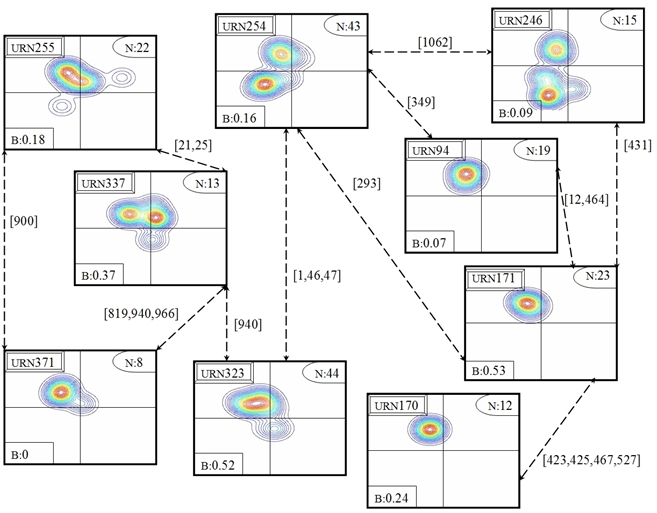
\includegraphics[width=.45\linewidth]{images/GeographicalNetworks.jpg}
%   \captionof{figure}{Geographical networks. Each box is an offender, displaying their codefendent links, and geographical range of offending.}
%   \label{fig:geonets}
% \end{minipage}%
% \begin{minipage}{.5\textwidth}
%   \centering
%   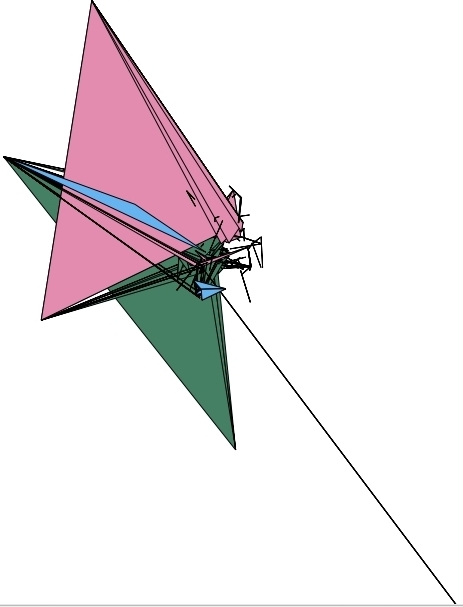
\includegraphics[width=.45\linewidth]{images/OffenderVictimOffenceTriples.jpg}
%   \captionof{figure}{Offender-Victim-Offence triples. Legend: woundings (light blue), murder (purple), manslaughter (dark blue), kidnapping (green), firearms offences (brown).}
%   \label{fig:offvictrips}
% \end{minipage}
% \end{figure}

Similar type modus operandi and the geographic and temporal data was
available for retail crime gangs in the north-east of
England~\cite{ewart+oatley:2009}. Retail crime is defined as
specifically stealing from retail outlets or shops. We were interested
in the most useful way of characterising a network or gang -- was it
perhaps on the basis of its membership (i.e. its stability, number,
type: family or not) or do gangs differ on the basis of their
geographical range and modi operandi, for instance falling into groups
such a `local', `travelling' or not.  We explored this by analysing
line connectivity and node connectivity over time for particular gangs
and the concepts of fragmentation, density, transitivity and
core/periphery structures (see Borgatti et
al.~\cite{borgatti-et-al:2009}).  Certainly it was intimated from
intelligence that within the data there were specialist and highly
organised gangs, for instance gangs from eastern Europe specialising
in purse theft, or a Malaysian gang targeting cheque fraud, or others
favouring mobile phone theft.


% TODO:
% This table is better suited to look like the above one, with 2 columns.
% Left column has three fields (spanning a few rows in certain cases): 
% Aggression / Modus operandi (what is stolen, from where and how) / Known associates and gang affiliations.
% Right column is all examples. 

%%% Insert Table 2 here
\begin{table}[!ht]
\centering
%\resizebox{0.9\textwidth}{!}{%
\begin{tabularx}{\textwidth}{|X|}
\hline
{\textbf{Aggression}} \\
\hline
NPI. Arrested Sunday [DATE] at TK Maxx, Ncle City Centre. Stole
clothing valued at \pounds 150.  Arrested [DATE] at M\&S, Newcastle,
for \pounds 20 theft.   DOESN'T LIKE BEING ARRESTED!!  MAY RESIST
VIOLENTLY. \\
\hline
{\textbf{Modus operandi (what is stolen, from where and how)}} \\
\hline
Thefts from TKMaxx v \pounds 90,  Eisenegger, v \pounds 64 and Sports
Connection v \pounds 62, all committed [DATE]. \\
\hline
Prolific. 31 Shopthefts recorded since [DATE].  Brief eg's - 240899
Kwik Save,Wallsend, \pounds 41 / 130599 Superdrug Ncle, \pounds 34 /
[CODE] HMV Ncle \pounds 49 / [CODE] Disney Store Ncle \pounds 15 /
[CODE] M\&S Ncle \pounds 144 \\
\hline
Arrested with [PERSON] on [DATE]Theft from HMV,Ncle,val \pounds 25,
Method -- One detags items,passes to other to conceal. Prev Shopthefts
'99 -  Fenwick [DATE]val \pounds 22 \& [DATE] val \pounds 5, Superdrug
[DATE] val \pounds 16, Boots v \pounds 17 , Bodyshop \pounds 5 \\
\hline
Sighting by [STAFF], Bhs, Ncle at 1705hrs [DATE]. Suspected attempt
Refund Fraud on trousers., val. \pounds 25. \\
\hline
At the close of a day's thieving/refunding he collects unused cheques
and cash proceeds of fraudulent refunds, having probably allowed
deductions for his cohorts' commission.  Well organised. Seen in
Curry's red Corsa – [NUMBERPLATE]. \\
\hline
Her last two thefts qualify Tams for a mention in this Target File. On
[DATE] She stole clothing from two Newcastle stores - River Island,
Eldon Sq (val.stolen \pounds 174) and Etams, (val.stolen \pounds 230)
she has used foil lined bags in the past. \\
\hline
Drug addict, [PERSON] is out daily stealing to feed his habit, and
usually steals DURACELL batteries which he can sell on for cash. He
has used baskets in Stores/Supermarkets and wanders around with
Duracell batteries hidden under a few groceries \\
\hline
Big value clothing theives using big foil lined bags. Make sure you
are aware of them because they are very active and very good at their
job. \\
\hline
{\textbf{Known associates and gang affiliations}} \\
\hline
Experienced shopthief and longstanding member of the [GANG], she has
recently been arrested together with [PERSON] and [PERSON] (her
Partner) on [DATE] for the usual BULK CLOTHING THEFT val.\pounds 684,
from Littlewoods, Metro Centre. \\
\hline
Thefts from Fenwick and C\&A [DATE] with [PERSON], [PERSON], [PERSON],
and [PERSON]. VAL \pounds 474\\
\hline
Prolific Shopthief in company with partner [PERSON] IDO XXX, in
Washington, Metrocentre and other Tyneside areas. \\
\hline
\end{tabularx}%}
\caption{Examples of intelligence related to retail crime.}
\label{tab:intelligence}
\end{table}


\section{Personality Theories}\label{personality}

\subsection{Detection (covertly) of personality type through game playing}\label{detectiongp}

A set rules of nine rules, representing the nine types of the
Enneagram personality typolology~\cite{newgent-et-al:2004}, was embedded in a game with various
`states' through which a user could navigate~\cite{oatleymsc:1996}; see
Figure~\ref{fig:sneakarch}. States in an `everyday life game' might
include: `{\emph{Getting ready for work}}', `{\emph{Taking an evening meal}}', `{\emph{Walking
through a park}}' and so on. States are linked according to real life,
so you can pass from `{\emph{Taking breakfast}}' to `{\emph{Travelling to work}}', but
not from the former to `{\emph{Taking an evening meal}}'. Questions are asked
of the user at each `state', the answers to which are known to
indicate evidence of a certain personality type. For instance, rules
for Types 2 and 5 are presented in Listings~\ref{lst:rule1} and
\ref{lst:rule2}. Importantly, the player is unaware that the game is
slowly determining their personality type (hence the name
SNEAK). SNEAK  actively searches for the nearest useful `states'
that can quickly lead to a classification, and plots a course
towards them. As each state follows coherently from the previous,
SNEAK presents the new states to the player, and the player is unaware
of the unfolding analysis.

This system was a rapidly developed prototype, to investigate the
extent of domain knowledge required to achieve a realistic
classification. Commenting on the system, an experienced Enneagram
practitioner said of Rule 1 that it was representative of the type but
that ``{\emph{...it could also possibly be a type2Giver. `sensingPerfection' is
too high a concept, probably something that the person is not normally
conscious of.}}'', and of Rule 5, that it was again representative,
``{\emph{but it is generally an easily recognisable type anyway, at least, by
themselves.}}''

The rules were simple, the states were contrived and of a
limited number, in order that every response from every type was able
to be coded. This is a long way from automatically diagnosing
someone's personality type through user interaction. Indeed, even for a
human, administering a personality interview is notoriously
difficult; for instance, the standard PCL-R assessment
procedure for psychopathy~\cite{hare:2003} requires a semi-structured interview and a
review of available file and collateral information. The purposes of
the interview include providing a sample of the individual's
interpersonal style, and allowing the user to compare and evaluate the
consistency of statements and responses, both within the interview and
between the interview and the collateral/file
information~\cite{hare:2003}.  Plutchick and
Conte~\cite{plutchick+conte:1989} confirm this difficulty: ``{\emph{A simple change in
test instructions e.g. `how do you feel now?' vs. `how do you usually
feel?' generally changes a mood measure into a personality trait
measure.}}''. Without significant structure it is hard to know what is being
assessed.

%%% Insert Fig 3 here
\begin{figure}[!ht]
\centering
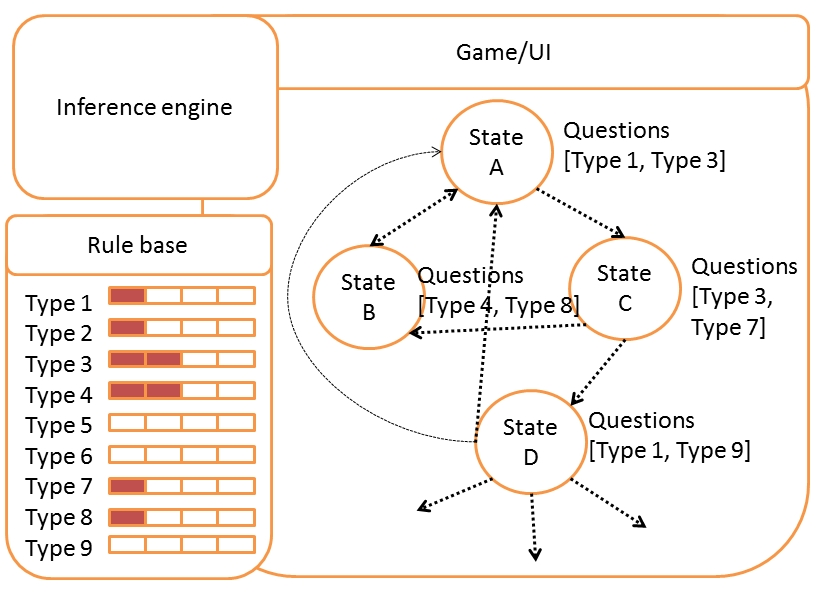
\includegraphics[width=0.8\columnwidth]{images/SNEAKarchitecture.jpg}
\caption{{\textbf{SNEAK architecture.}} The rules/classifications are partially instantiated. SNEAK will direct the user to a question that will differentiate between the two most likely current classifications (Type 3 and 4). }
\label{fig:sneakarch} 
\end{figure}

%%% Insert Listing 1 and Listing 2 here
\noindent\begin{minipage}{.48\textwidth}
\begin{lstlisting}[caption=Rule for Type 1 Perfectionist,frame=none,basicstyle=\ttfamily\scriptsize,label=lst:rule1]
Rule1:if
 (Person isa avoidAnger,A) and
 (Person isa postponePleasure,B) and
 (Person isa tryToBeGood,C) and
 (Person isa sensingPerfection,D)
 then
 (Person isa type1Perfectionist,E).
\end{lstlisting}
\end{minipage}\hfill
\begin{minipage}{.48\textwidth}
\begin{lstlisting}[caption=Rule for Type 5 Observer,frame=none,basicstyle=\ttfamily\scriptsize,label=lst:rule2]
Rule5:if
 (Person isa needTimeToReflect,A) and
 (Person isa drainedByCommittment,B) and
 (Person isa greedyForKnowledge,C) and
 (Person isa detachesAttentionToImpartiallyObserve,D)
 then
 (Person isa type5Observer,E).
\end{lstlisting}
\end{minipage}



\subsection{Detection of personality traits through textual analysis
  of social network data}\label{detection}

Advances in psychology research have suggested it may be
possible to classify personality through usage of textual analysis of
social networking sites rather than the traditional approaches such as
interviews or survey self-completion. Studies in the USA have
suggested certain key words and phrases can signal underlying
tendencies and that this can form the basis of identifying certain
aspects of personality~\cite{woodworth-et-al:2012}. Extrapolating
forward suggests that by investigation of an individual's online
comments it maybe possible to identify individuals personality
traits. Initial evidence in support of this hypothesis was
demonstrated in 2012 by a study which analysed Twitter data for
signs of psychotic behaviour in respondents~\cite{sumner-et-al:2012}.

There have been many studies relating to personality and language
using the Five Factor model of
personality~\cite{pennebaker+king:1999,oberlander+gill:2004,oberlander+gill:2006,iacobelli-et-al:2011}.
However, the Five Factor model has known
limits~\cite{eysenck:1992,paunonen+jackson:2000,block:2010}: it has
been criticised for its limited scope, methodology and the absence of
an underlying theory, and attempts to replicate the Five Factor model
in other countries with local dictionaries have succeeded in some
countries but not in
others~\cite{szirmak+deraad:1994,defruyt-et-al:2004}. Additionally,
while Costa and McCrae~\cite{costa+mccrae:1992} claim that their Five
Factor model ``represents basic dimensions of personality'',
psychologists have identified important trait models, for instance
Cattell's 16 Personality Factors~\cite{cattell:1946} and Eysenck's
biologically based theory~\cite{eysenck:1947}. However, as discussed
previously, this model has a significant body of research, which
provides useful context for studies.

We have used a top-down dictionary
approach~\cite{oberlander+gill:2006}, as opposed to a bottom-up
method, such as collection of words and n-grams. We use two standard
psycholinguistic dictionaries: LIWC~\footnote{Linguistic Inquiry and
Word Count.  Pennebaker and King~\cite{pennebaker+king:1999} discuss
the individual differences in linguistic styles, and developed the
LIWC tool to try and measure these. Their text analysis software
calculates the degree to which people use different categories of
word, determining the degree any text uses positive or negative
emotions, self-references, causal words, and 70 other language
dimensions.} and MRC~\footnote{The MRC Psycholinguistic Database is a
machine-usable dictionary containing 150,837 words with up to 26
linguistic and psycholinguistic attributes for each -- psychological
measures are recorded for only about 2500 words. This data was
empirically derived, which differs from the human judgment of
psychological categories that created the LIWC.}, and the equations
based upon these features, for the Five Factors, based upon the work
of Mairesse et al.~\cite{mairesse-et-al:2007}. MRC category
{\texttt{K\_F\_NSAMP}} is the Kucera-Francis number of samples (from
the Brown Corpus analysis), LIWC categories {\texttt{UNIQUE}},
{\texttt{ABBREVIATIONS}} and {\texttt{PRONOUN}} are the number of unique
words, abbreviations and pronouns respectively, and {\texttt{HEARING}}
is a count of words such as `heard', `listen', `sound'. An example
equation is presented in Listing~\ref{lst:mrcliwc}.

%%% Insert Listing 3 here
\begin{lstlisting}[caption={Equation relating to extraversion psychological trait, based on MRC and LIWC
  psycholinguistic features.},frame=none,basicstyle=\ttfamily\footnotesize,label=lst:mrcliwc]
  Extraversion =
     -0.0379 * MRC.K_F_NSAMP +  -0.0803 * LIWC.UNIQUE +  -0.6074 *  LIWC.ABBREVIATIONS +   0.1445 * LIWC.PRONOUN +  -0.3941 * LIWC.HEARING + 17.1407;
\end{lstlisting}

The data that we have used for this study is from Twitter, and specifically looks at a person's
retweet count. This tag is an unofficial way to provide
attribution to the original publisher. If a person wishes to share a tweet
from someone else (irrespective of whether they agree or disagree with
it), it is possible to re-tweet it and share it on their own Twitter
timeline. The retweet count provides the number of times
that the tweet has been re-tweeted.

Therefore, a retweet count of zero means the tweet is authored by the
user, whereas a value greater than zero means that someone else
authored the tweet, although the user has shared the content. A count
of zero indicates the user's own words and sentiments, a count greater
than zero indicates other's words. Of course we can make further
categories, for instance a count of 1 will indicate people being
directly followed, and much larger counts will indicate very popular
sentiments, and so on. However for this study, we consider only these
two categories. In this way, for a single user, we have two different
chunks of text, aggregated self-authored tweets and aggregated
followed tweets. We perform our Five Factor analysis on these, giving
two sets of Five Factor results for each user. In future work we will
use multi-dimensional scaling to work out an algorithmic difference
between users; however for this study we have selected Chernoff
faces~\cite{chernoff:1973} for the visual representation. The Five
Factors are displayed as five features on a stylised
face. Figure~\ref{fig:chernoff} shows the Chernoff face representation
of the Five Factors (using the R language with the {\emph{aplpack}}
library). A specific facial feature represents each one of the
factors. Additionally the height of face (extraversion) has an
additional impact also on the colour of the face, the width of eyes
influences the eye colour, the width of hair affects the colour of the
hair, and the width of nose effects the colour of nose.

%%% Insert Fig 4 and Fig 5 here
% \begin{figure}
% \centering
% \begin{minipage}{.33\textwidth}
%   \centering
%   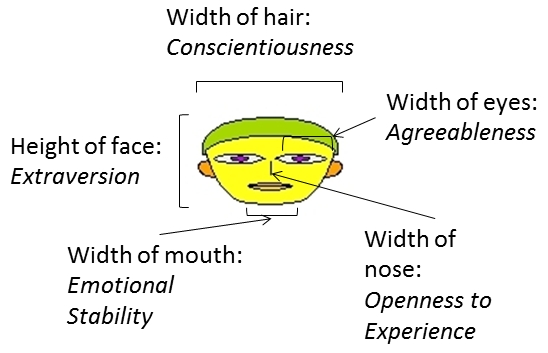
\includegraphics[width=.33\linewidth]{images/MeanChernoffFace.jpg}
%   \captionof{figure}{{\textbf{``Mean'' Chernoff face with Five Factor dimensions labelled.}}}
%   \label{fig:chernoff}
% \end{minipage}%
% \begin{minipage}{.65\textwidth}
%   \centering
%   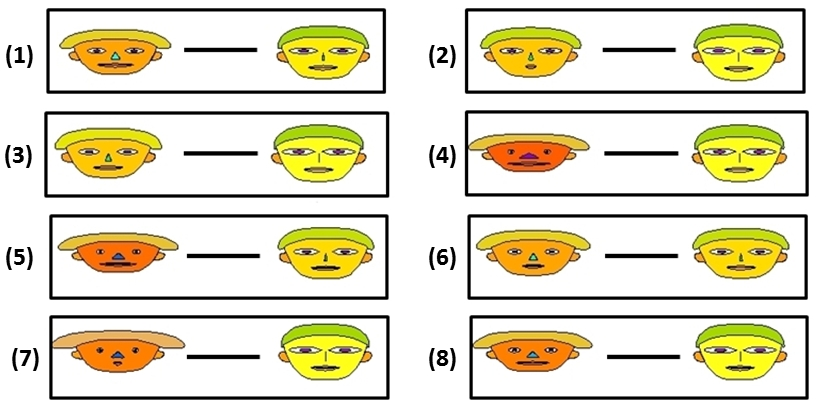
\includegraphics[width=.65\linewidth]{images/PairsOfBehaviour.jpg}
%   \captionof{figure}{{\textbf{Pairs of behaviour for a user.}} Left image of each pair is self-authored, i.e. self-image, and right image is other-authored but liked.}
%   \label{fig:pairsofbehav}
% \end{minipage}
% \end{figure}


\begin{figure}[!ht]
\centering
  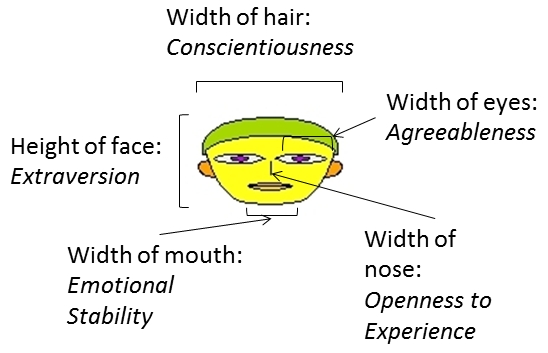
\includegraphics[width=0.7\textwidth]{images/MeanChernoffFace.jpg}
  \captionof{figure}{{\textbf{``Mean'' Chernoff face labelled with dimensions.}}}
  \label{fig:chernoff}
\end{figure}

% other refs: ~\cite{john-et-al:1991}; ~\cite{jonason+webster:2010};
% ~\cite{petrides+furnham:2006}; ~\cite{aluja-et-al:2003}
The sample used undergraduate students (n=47) that engaged with a
study (to be reported) looking at the correlation between social media
profiles (Twitter, Facebook, LinkedIn) and personality typology and
affect questionnaires: 44-item Big-Five Inventory, 12-item Dark Triad
inventory, 30-item Trait Emotional Intelligence Questionnaire (Short
Form), 144-item Riso-Hudson Enneagram Type Indicator Version 2.5 and
48-item Eysenck Personality Questionnaire--revised (Short Scale). We
have only presented eight profiles in Figure~\ref{fig:pairsofbehav},
deliberately choosing profiles that present significant differences
between the self-authored and other-authored faces.

\begin{figure}[!ht]
\centering
  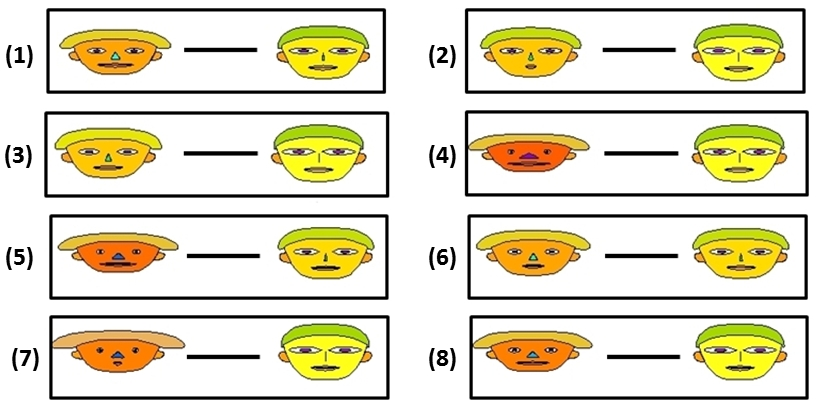
\includegraphics[width=0.9\textwidth]{images/PairsOfBehaviour.jpg}
  \captionof{figure}{{\textbf{Pairs of behaviour for a user.}} Left image of each pair is self-authored, i.e. self-image, and right image is other-authored but liked.}
  \label{fig:pairsofbehav}
\end{figure}


\section{Conclusions}
While we have to be cautious about what we deduce in relation to
criminal profiling~\cite{alison-et-al:2002,snook-et-al:2008}, there is
no doubt it is possible to determine certain traits of operational
value from structured analysis of data from crime investigations. This
will be equally true of data aggregated from other sources. Different
data lends itself to different forms of analysis. In some
circumstances traits and affects can be revealed, in others perhaps
even the beliefs, opinions, or notions of identity (McAdams' top and
middle levels).

This paper has presented a wide range of operational data and
modelling techniques.  These have differed with respect to the degree
of knowledge inherent in the data itself, the sophistication of the
modelling technique and the difficulty of the operational inference.
The geospatial and network data (and their standard modelling
techniques) are sufficient to characterise certain features of
operational usefulness (matching crimes in an area, identifying
possible accomplices, determining local versus travelling criminals),
but barely reaching McAdams' trait level.  Modus operandi data
contains greater potential for psychological modelling, for instance
whether someone is careful, risk averse, capable of violence,
possessing a degree of craft, all indicating traits.  The rule-based
personality game illustrated the need for a heavily indexed and
tightly constrained knowledge to detect personality features best
described as McAdams' middle and even highest level.  Finally the
textual data from Twitter was sufficient to apply psycholinguistic
techniques (although we are not able in this paper to consider the
limitations of the approach), revealing personality trait knowledge
(McAdams' lowest level). The technique (and future use of
multi-dimensional scaling) shows how different high level profiles for
an individual can be computed and visualised.
 
It is hoped that with additional knowledge sources, and solutions from
the converging fields of psychology and personality, mindfulness and
psychoanalysis, with computer-based models (for instance, using
belief-desire-intention (BDI) agents and life-logging) that this field
will develop significantly in the future.


\bibliographystyle{splncs}
%\bibliography{hcii2014}

\begin{thebibliography}{10}

\bibitem{vazire+gosling:2004}
Vazire, S., Gosling, S.D.:
\newblock {e-Perceptions: Personality Impressions Based on Personal Websites}.
\newblock {Journal of Personality and Social Psychology} \textbf{87}(1) (2004)
  123--132

\bibitem{haggerty-et-al:2012}
Haggerty, J., Casson, M.C., Haggerty, S., Taylor, M.J.:
\newblock {A Framework for the Forensic Analysis of User Interaction with
  Social Media}.
\newblock {International Journal of Digital Crime and Forensics} \textbf{4}(4)
  (2012)  15--30

\bibitem{adams:1996}
McAdams, D.P.:
\newblock {Personality, Modernity, and the Storied Self: A Contemporary
  Framework for Studying Persons}.
\newblock {Psychological Inquiry} \textbf{7}(4) (1996)  295--321

\bibitem{gosling:2009}
Gosling, S.:
\newblock {Snoop: What Your Stuff Says About You}.
\newblock {Profile Books} (2009)

\bibitem{costa+mccrae:1992}
Costa, P.T., McCrae, R.R.:
\newblock {Neo PI-R Professional Manual}.
\newblock {Psychological Assessment Resources}. (1992)

\bibitem{norman:1963}
Norman, W.T.:
\newblock {Toward an adequate taxonomy of personality attributes: Replicated
  factor structure in peer nomination personality ratings}.
\newblock {Journal of Abnormal and Social Psychology} \textbf{66}(6) (1963)
  574--583

\bibitem{mairesse-et-al:2007}
Mairesse, F., Walker, M.A., Mehi, M.R., Moore, R.K.:
\newblock {Using Linguistic Cues for the Automatic Recognition of Personality
  in Conversation and Text}.
\newblock {Journal of Artificial Intelligence Research} \textbf{30} (2007)
  457--500

\bibitem{oatley+ewart:2003}
Oatley, G.C., Ewart, B.W.:
\newblock {Crimes Analysis Software: `Pins in Maps', Clustering and Bayes Net
  Prediction}.
\newblock {Expert Systems with Applications} \textbf{25}(4) (2003)  569--588

\bibitem{oatley-et-al:2006a}
Oatley, G.C., McGarry, K., Ewart, B.W.:
\newblock {Offender Network Metrics}.
\newblock {WSEAS Transactions on Information Science \& Applications}
  \textbf{12}(3) (2006)  2440--2448

\bibitem{oatley-et-al:2006b}
Oatley, G.C., Ewart, B.W., Zeleznikow, J.:
\newblock Decision support systems for police: Lessons from the application of
  data mining techniques to ``soft'' forensic evidence.
\newblock {Artificial Intelligence and Law} \textbf{14}(1-2) (2006)  35--100

\bibitem{ewart+oatley:2003}
Oatley, G.C., Ewart, B.W.:
\newblock {Applying the concept of revictimisation -- using burglars' behaviour
  to predict houses at risk of future victimisations}.
\newblock {International Journal of Police Science and Management}
  \textbf{5}(2) (2003)  69--84

\bibitem{ewart+oatley:2009}
Ewart, B.W., Oatley, G.C.:
\newblock {The criminal patterns of retail offending gangs: Some lessons from
  the integration of social network and geographical analyses}.
\newblock In: Proceedings of the British Psychological Society's Division of
  Forensic Psychology Conference. (2009)

\bibitem{borgatti-et-al:2009}
Borgatti, S.P., Mehra, A., Brass, D.J., Labianca, G.:
\newblock {Network Analysis in the Social Sciences}.
\newblock {Science} \textbf{323}(5916) (2009)  892--895

\bibitem{newgent-et-al:2004}
Newgent, R.A., Parr, P.E., Newman, I., Higgins, K.K.:
\newblock {The Riso-Hudson Enneagram Type Indicator: Estimates of Reliability
  and Validity}.
\newblock {Measurement and Evaluation in Counseling and Development}
  \textbf{36}(4) (2004)  226--237

\bibitem{oatleymsc:1996}
Oatley, G.C.:
\newblock Computer implementation of indirect questioning techniques for
  psychological testing.
\newblock Master's thesis, University of Westminster (1996)

\bibitem{hare:2003}
Hare, R.D.:
\newblock {Hare Psychopathy Checklist-Revised (PCL-R)}.
\newblock Pearson. 2nd edn. (2003)

\bibitem{plutchick+conte:1989}
Plutchick, R., Conte, H.R.:
\newblock {Measuring emotions and the derivatives of the emotions: Personality
  traits, ego defenses and coping styles}.
\newblock In: {Contemporary Approaches to Psychological Assessment}. Brunner
  Maze (1989)  239--269

\bibitem{woodworth-et-al:2012}
Woodworth, M., Hancock, J., Porter, S., Hare, R., Logan, M., O’Toole, M.E.,
  Smith, S.:
\newblock {The Language of Psychopaths: New Findings and Implications for Law
  Enforcement}.
\newblock FBI Law Enforcement Bulletin (July 2012)

\bibitem{sumner-et-al:2012}
Sumner, C., Byers, A., Boochever, R., Park, G.J.:
\newblock {Predicting Dark Triad Personality Traits from Twitter Usage and a
  Linguistic Analysis of Tweets}.
\newblock In: {Proceedings of the 11th International Conference on Machine
  Learning and Applications (ICMLA 2012)}, IEEE Press (2012)

\bibitem{pennebaker+king:1999}
Pennebaker, J.W., King, L.A.:
\newblock {Linguistic styles: language use as an individual difference}.
\newblock {Journal of Personality and Social Psychology} \textbf{77} (1999)
  1296–1312

\bibitem{oberlander+gill:2004}
Oberlander, J., Gill, A.J.:
\newblock {Individual differences and implicit language: Personality,
  parts-of-speech and pervasiveness}.
\newblock In: {Proceedings of the 26th Annual Conference of the Cognitive
  Science Society}. (2004)  1035--1040

\bibitem{oberlander+gill:2006}
Oberlander, J., Gill, A.J.:
\newblock {Language with character: A stratified corpus comparison of
  individual differences in e-mail communication}.
\newblock {Discourse Processes} \textbf{42}(3) (2006)  239--270

\bibitem{iacobelli-et-al:2011}
Iacobelli, F., Gill, A.J., Nowson, S., Oberlander, J.:
\newblock {Large Scale Personality Classification of Bloggers}.
\newblock In: {Proceedings of the 4th International Conference on Affective
  Computing and Intelligent Interaction (ACII'11)}, Springer (2011)  568--577

\bibitem{eysenck:1992}
Eysenck, H.J.:
\newblock {Four ways five factors are not basic}.
\newblock {Personality and Individual Differences} \textbf{13}(6) (1992)
  667--673

\bibitem{paunonen+jackson:2000}
Paunonen, S.V., Jackson, D.N.:
\newblock {What is beyond the Big Five? Plenty!}
\newblock {Journal of Personality} \textbf{68}(5) (2000)  821--836

\bibitem{block:2010}
Block, J.:
\newblock {The Five-Factor Framing of Personality and Beyond: Some
  Ruminations}.
\newblock {Psychological Inquiry} \textbf{21}(1) (2010)  2--25

\bibitem{szirmak+deraad:1994}
Szirm\'{a}k, Z., {De Raad}, B.:
\newblock {Taxonomy and structure of Hungarian personality traits}.
\newblock {European Journal of Personality} \textbf{8}(2) (1994)  95--117

\bibitem{defruyt-et-al:2004}
{De Fruyt}, F., McCrae, R.R., Szirm\'{a}k, Z., Nagy, J.:
\newblock {The Five-Factor Personality Inventory as a Measure of the
  Five-Factor Model: Belgian, American, and Hungarian Comparisons with the
  NEO-PI-R}.
\newblock {Assessment} \textbf{11}(3) (2004)  207--215

\bibitem{cattell:1946}
Cattell, R.B.:
\newblock The description and measurement of personality.
\newblock Harcourt, Brace \& World (1946)

\bibitem{eysenck:1947}
Eysenck, H.J.:
\newblock {Dimensions of Personality}.
\newblock Routledge \& Kegan Paul (1947)

\bibitem{chernoff:1973}
Chernoff, H.:
\newblock {The Use of Faces to Represent Points in k-Dimensional Space
  Graphically}.
\newblock {Journal of the American Statistical Association} \textbf{68}(342)
  (1973)  361--368

\bibitem{alison-et-al:2002}
Alison, L., Bennell, C., Mokros, A., Ormerod, D.:
\newblock {The Personality paradox in offender profiling. A theoretical review
  of the processes involved in deriving background characterictics from crime
  scene actions}.
\newblock {Psychology, Public Policy, and Law} \textbf{8}(1) (2002)  115--135

\bibitem{snook-et-al:2008}
Snook, B., Cullen, R.M., Bennell, C., Taylor, P.J., Gendreau, P.:
\newblock {The Criminal Profiling Illusion: What's Behind the Smoke and
  Mirrors?}
\newblock {Criminal Justice and Behavior} \textbf{35}(10) (2008)  1257--1276

\end{thebibliography}

\end{document}
